\Chapter{Kamerapozíció becslése a virtuális térben}

\Section{Markerek}

\SubSection{Klasszikus markeres megoldások}\\
A kiterjeszetett valóság fontos eszköze a marker, ami a model/modellek térben való elhelyezésében segít. Számos nyílt forráskodú könytár rendelkezésre áll a klasszikus értelemben vett markerekből.\\

{\bf Vonalkód, QR-kód:}\\
„A  QR  kód vagyis Quick  Response  (gyors  válasz) egy  mátrix  vonalkód,  vagy  más  néven kétdimenziós kód, mely intelligensebb, több információt hordoz magában a vonalkódoknál: míg egy vonalkód mintegy 13 számjegyet tárol, addig a QR kód 7000 számot és 4300 alfanumerikus karaktert illetve weboldalak címeit (URL),nagy terjedelmű szöveget és telefonszámokat is képes tárolni, bármilyen nyelven.”\\

\begin{figure}[htp]
    \centering
   	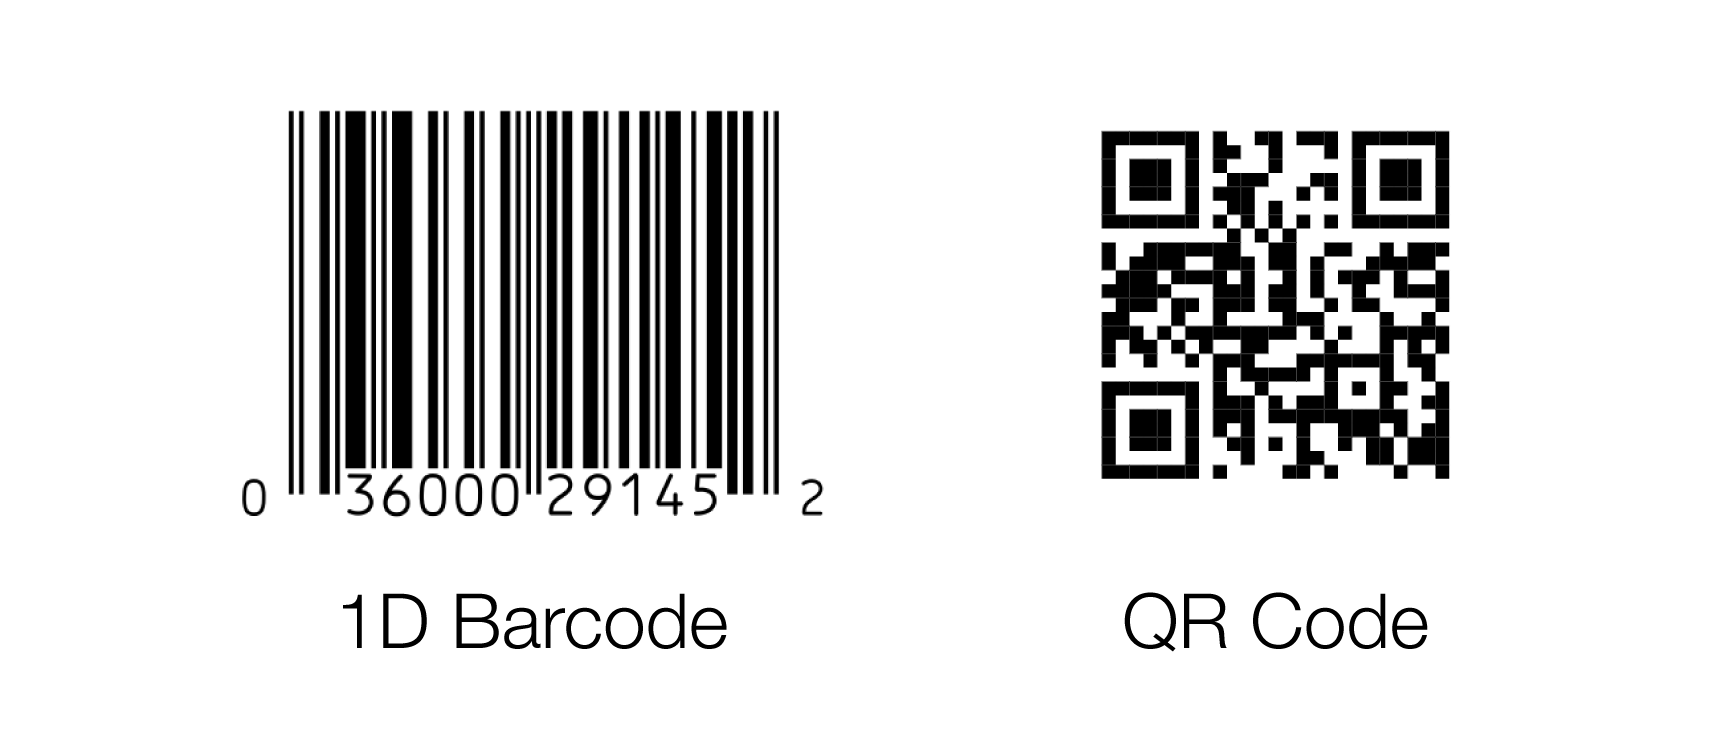
\includegraphics[width=4.8truecm, height=2truecm]{images/qr_bar.png}
	\caption{Vonalkód, QR-kód}
\end{figure}

{\bf „Keretes” markerek:}

Az ilyen típusú markerek két részből állnak; egy fekete keretből, ami a felismerést segití és egy belső mintából. A belső minta lehet kép, egyedi bináris minta, valami azonosítja a markert, információt hordoz.

A keret fontos szerepet tölt be, hisz egy fekete téglalapot/négyzetet viszonylag egyszerűen és gyorsan fel lehet ismerni egy képen, meghatározni annak pozícióját a kamerához képest, sarok pontjait, a középpontját.

Ilyen típusú marker például az ARToolKit marker (középen egy kép van, ami bináris képként lesz kezelve), ARTag, AprilTag, ArUco. (mindháromnál egy bináris minta van középen)

Kombinálni is szokták az egyszerűbb markereket: a QR-kódot és a kerettel rendelkező markereket, vagy a QR kód van a keret belsejében vagy pedig a QR kód közepén szerepel például egy ArUco marker vagy egy kép (pl.VuMark).

\begin{figure}[htp]
    \centering
   	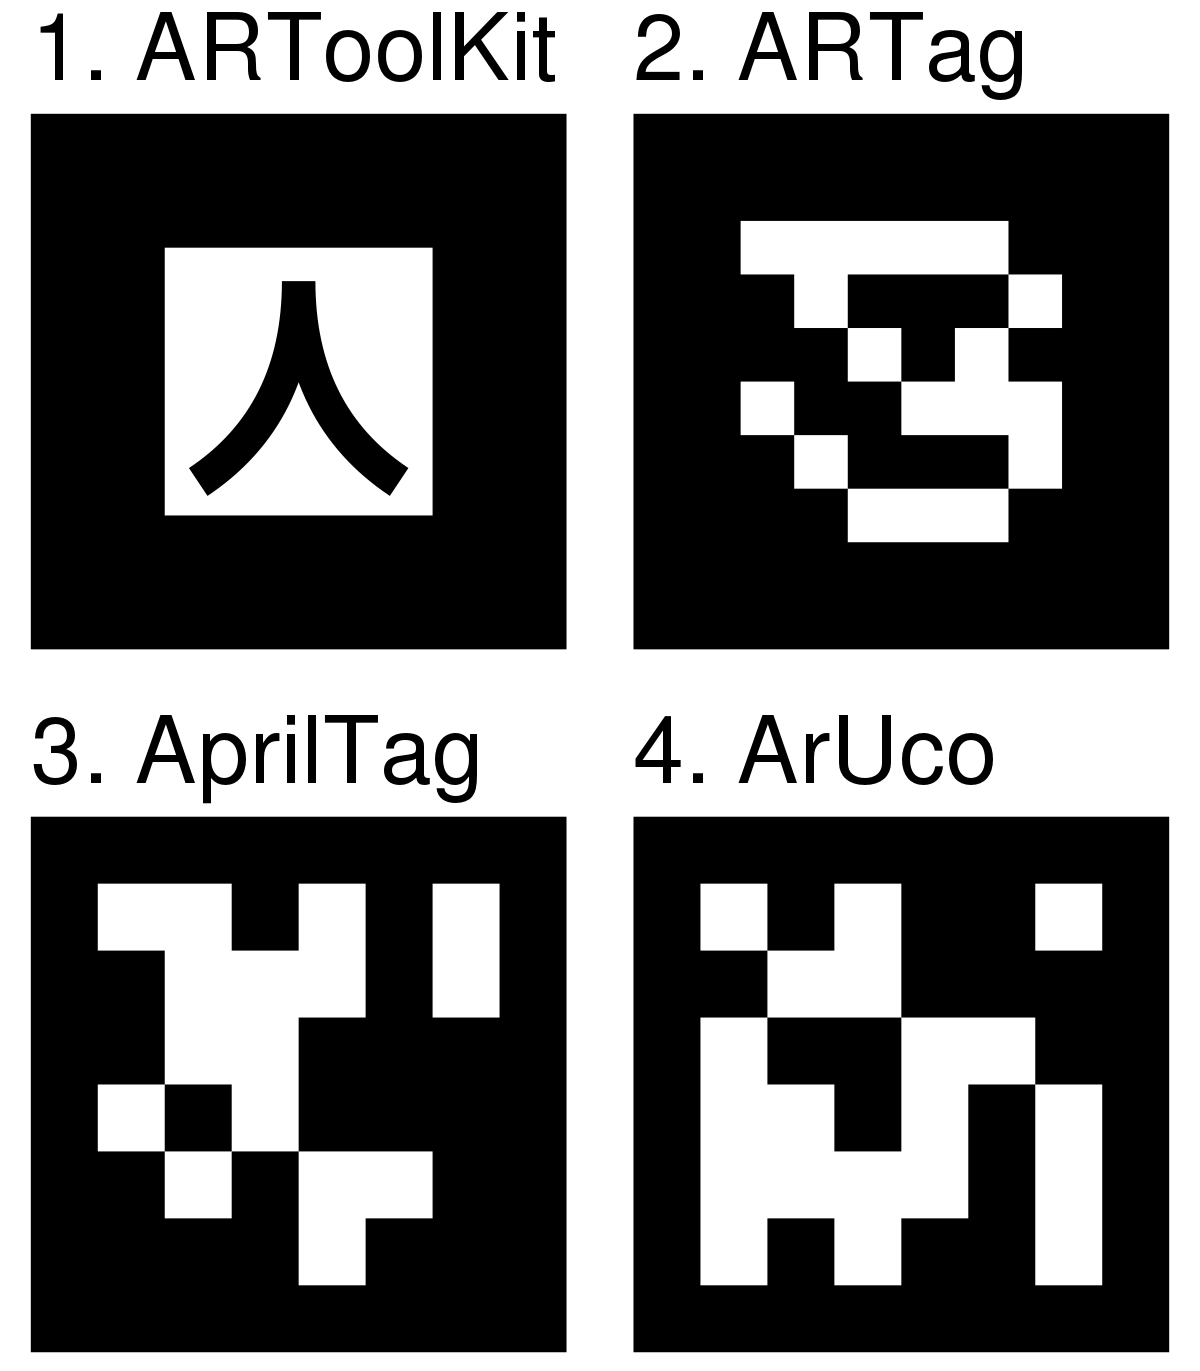
\includegraphics[width=3truecm, height=3truecm]{images/markerek.png}
	\caption{ArToolKit, ARTag, AprilTag, ArUco}
\end{figure}


\SubSection{Betanítható markerek}

A kiterjesztett valóság technikai fejlődéssel a markerek is bonyolultabbá váltak, lehetőség nyílt hétköznapi tárgyak, épületek és egyéb dolgok markerként kezelésére.

Természetesen ezek detektálása nehezebb, illetve betanítást igényel.

Léteznek továbbá úgynevezett marker nélküli (markerless) AR alkalmazások is, a szenzorok felmérik környezetet és megfelelő helyre pozicionálják a megjelenítendő objektumot/objektumokat. (pl. földrajzi koordináták felhasználása: PokemonGO)

\Section{Inerciális szenzorok}

A fejlettebb telefonokban található inerciális szenzorok fontosak a kiterjeszett valóság felhasználásával készült alkalmazások müködtetéséhez.  

Az inerciális szenzorok gyorsulásérzékelőkből és giroszkópokból állnak, minél nagyobb a számuk, annál pontosabb eredményeket képesek biztosítani.

Az inerciális szenzorokkkal a telefon térbeli helyzetének és annak változára vonatkozó adatokat kaphatunk meg.

Az accelerométer a telefon helyzetének változását méri a x, y és y tengelyeket alapul véve. 

A telefonokban található giroszkóp (vagy gyro szenzor) a gyorsulásmérő egy fejletebb verziója.
Míg accelerometer tengely alapú elmozdulást mér, addig a giroszkóp az acceletométert felhasználva minden apró változást érzékel. Pontosabb adatokat kaphatunk vele.

\begin{figure}[htp]
    \centering
   	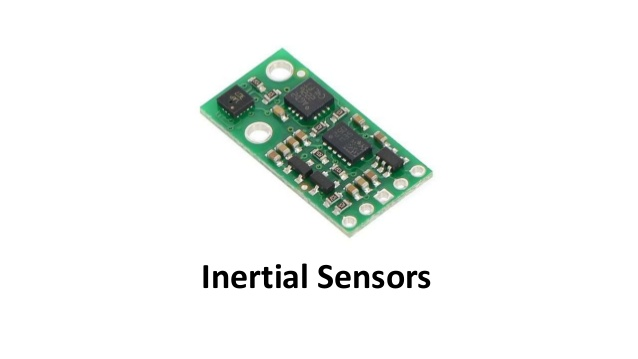
\includegraphics[width=3truecm, height=2truecm]{images/inertial.jpg}
	\caption{inerciális szenzor}
\end{figure}


\Section{Az Aruco marker használata}

Az ArUco (Augmented Reality University of Cordoba) markereket 2014-ben fejlesztette ki kollégáival S.Garrido-Jurado Spanyolországban. 

Az ArUco könyvtár nyílt forráskódú és C++ nyelven íródott, OpenCV alapú. 

Ar ArUco markerek két részből állnak, egy fekete keretből és az egyedi bináris mintából, ami azonosítja a markert. 

Az OpenCV-s támogatottsága miatt került kiválasztásra a dolgozathoz. A detektálást számos beépített függvény segíti.\\

\begin{figure}[htp]
    \centering
   	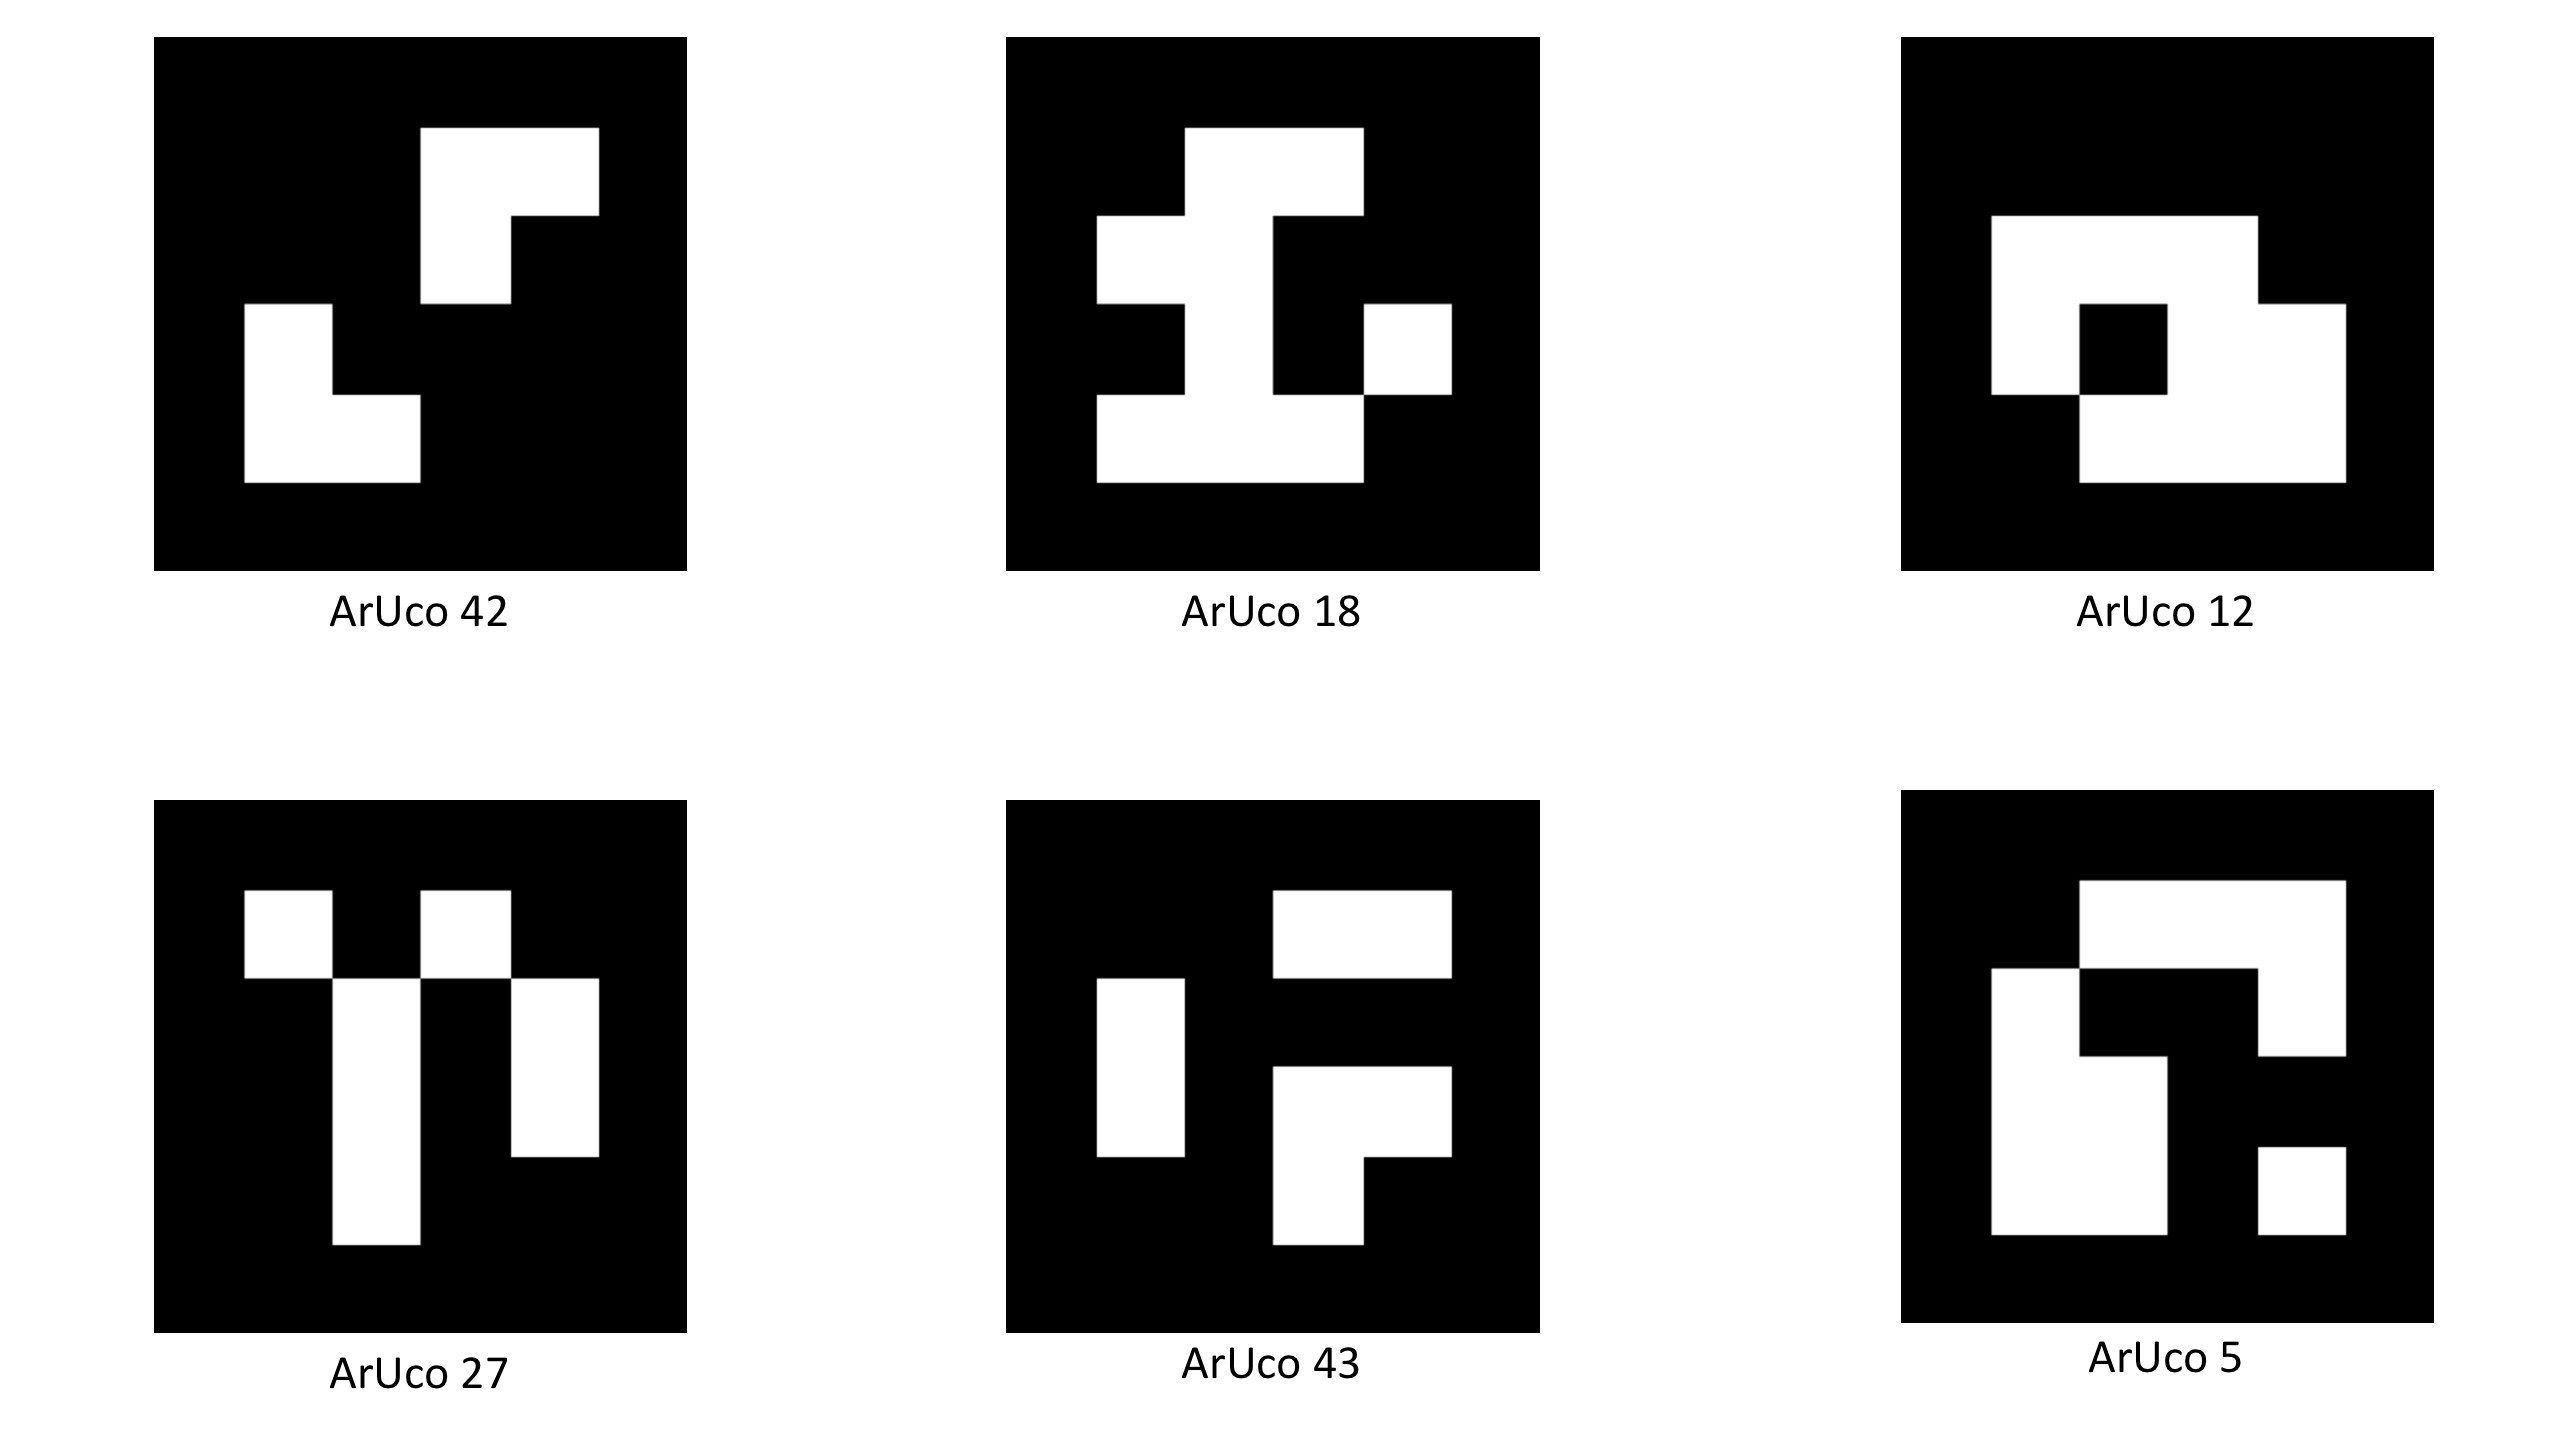
\includegraphics[width=4.8truecm, height=3truecm]{images/kep.png}
	\caption{Aruco markerek a 4X4-es könyvtárból}
\end{figure}

\SubSection{Típusai, használati módok}

Az ArUco markerek különböző könyvtárak érhetőek el, a marker méretében (szükséges bitek száma), belső minta oszlop és sor számában (az oszlop és sor szám mindig megegyezik) és az elérhető azonosítók számában térnek el.


A bináris minta 4x4-től a 7x7 bitig terjed, ebbe nem számít bele a keret.

Azonban minél bonyolultabb egy minta és minél nagyobb annál nehezen felismerni, ezért én a  \texttt{DICT\_4X4\_100}-t használtam.

Ahol a a \texttt{\_4x4} a bitek száma \texttt{100} pedig a könyvtárban lévő markerek azonosítóit jelöli.
Ez azt jelenti, hogy az azonosítók  0 és 99 között vannak.

\SubSection{Kamera kalibrálása}

% TODO: https://medium.com/@aliyasineser/aruco-marker-tracking-with-opencv-8cb844c26628

A kamera kalibrációjához 6x9-es sakktábla mintát használtam. (A külső sáv nem számolandó bele, az a felismerést könnyíti, a belső minta számít.) 

A kalibráció eredményességéhez a négyzeteknek szabályosnak, egyformának kell lenniük és fontos, hogy a nyomtatás során a minta ne torzuljon el, ne legyen átméretezve. 

A pontosság növelése érdekében a képeket érdemes minél változatosabb szögben és távolságból elkészíteni. Valamint ügyelni kell arra, hogy a lap egyenes legyen tartva, ezért célszerű megfelelő támaszt használni hozzá.

A kalibráció során kapjuk meg a későbbiekben nélkülözhetetlen együttható (kamera) mátrixot, a disztorziós együtthatókat, az eltolási és forgatási vektorokat.

A kalibrációt végző függvénynek a sorok és oszlopok számára, a négyzetek oldalhosszára és a fent említett képekre van szüksége.

A folyamat során meg kell határozni a fekete-fehérré tett képen szereplő a sakktábla minta sarokpontjait 
\texttt{findChessboardCorners()} függvénnyel, pontosabbá tenni azok koordinátáit 
\texttt{cornerSubPix()} -lel. 
\begin{python}
ret, corners = cv2.findChessboardCorners(gray, (width, height), None)
...
corners2 = cv2.cornerSubPix(gray, corners, (11, 11), (-1, -1), criteria)
\end{python} 

Majd ezen pontokat, (projekciós pontjai a sakktáblába mintának) a objektum pontjait ( a minta pontjai a minta terében), a kép méretét kell megadni \texttt{calibrateCamera()} függvénynek. \\

\begin{python}
  ret, mtx, dist, rvecs, tvecs = cv2.calibrateCamera(objpoints,
   imgpoints, gray.shape[::-1], None, None)
\end{python} 

A kimenetei a függvénynek:
\begin{itemize}
\item {\bf cameraMatrix}: $3 \times 3$ lebegőpontos kamera matrix
\[
A = 
\begin{bmatrix}
	f_x & 0 & 0 \\
	0 & f_y & 0 \\
	0 & 0 & f_z \\
\end{bmatrix}
\]

\item {\bf distortionCoefficient}: Bemeneti/kimenti torzítási együttható vektora:
\[
(k_1, k_2, p_1, p_2, [, k_3 [, k_4, k_5, k_6, [, s_1, s_2, s_3, s_4 [, \tau_x, \tau_y]]]])
\]
4, 5, 8, 12 vagy 14 elemből állhat.

\item {\bf rvecs}: A mintákhoz tartozó elforgatási vektorok becsült kimeneti vektora.

\item {\bf tvecs}  A mintákhoz tartozó vektorok becsült kimeneti vektor
\end{itemize}


\begin{figure}[htp]
    \centering
   	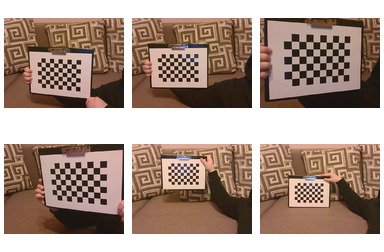
\includegraphics[width=7truecm, height=6truecm]{images/calibration.jpg}
	\caption{Kalibráláshoz használt képek közül néhány}
\end{figure}


\SubSection{Demo alkalmazás}

A markerek detektálásának eredményességét befolyásolja a fényviszony, a kamerához viszonyított pozíció, a minta bonyolultsága, a szög amiben látszik és a mérete. Továbbá óriási hátrány, hogy ha takarásra kerül egy része a markernek (legyen ez akármilyen kicsi), akkor nem lesz felismerhető.

Az ArUco marker felismerésére használt demó alkalmazás bekalibrálja a kamerát (ha ez még nem történt meg), majd a kalibrációból kapott \texttt{camera\_matrix} és a \texttt{dist\_Coefficient} felhasználásával detektálja a markert az élő képen.

A folyamatos kapcsolat érdekében végtelen ciklust indul.
Ezután kapcsolatot kell teremteni a kamerával és mindig az adott pillanatnyi képpel dolgozni. 
Ehhez az OpenCv \texttt{VideoCapture} függvényére van szükség. A 0 a laptop saját beépített kameráját jelöli , ha csatlakoztatható USB-s kamerával szeretnénk dolgozni, akkor az 1 paramétert kell megadni.

\begin{python}
cap = cv2.VideoCapture(0)
...
ret, frame = cap.read()
\end{python}
A kamera kép olvasásakor visszakapott második paraméterre lesz szükségünk, ami maga a kép. Ha valamilyen okból kifolyólag nem sikerül olvasni, akkor hamis értékkel és üres képpel tér vissza.

Ha meg van a kép, meg kell adni a megfelelő könyvtárat, amiben szerepel a marker, amit fel akarunk ismerni. Jelen esetben ez  \texttt{DICT\_4X4\_100}.
\begin{python}
aruco_dict = aruco.Dictionary_get(aruco.\texttt{DICT\_4X4\_100})
\end{python}

Majd ezt a változót,a paramétereket, a képet, a kamera mátrixot és disztorziós együtthatókat felhasználva detektáljuk a markert a \texttt{aruco.detectMarker()} függvény segítségével.

\begin{python}
corners, ids, rejectedImgPoints = aruco.detectMarkers(image, aruco_dict,
parameters=parameters,
cameraMatrix=mtx,
distCoeff=dist)
\end{python}

Eredményként a megtalált markerek sarokpontjait és a belső minta által definiált id-kat kapjuk vissza.

A sarokpontokat és a kamera mátrixot és a disztorziós együtthatót felhasználva a 
\texttt{estimatePoseSingleMarkers} meghatározza a marker elfordulását és eltolását kamerához képest. 

Ezután  mindenezt felhasználva a képen talált markert a program  körbe rajzolja, kijelöli a felső sarok pontját és ráteszi a képre marker koordináta rendszeréhez tartozó triédert.\\

\begin{python}
rvec, tvec ,_ = aruco.estimatePoseSingleMarkers(corners,
0.17, matrix_coefficients, distortion_coefficients)       
aruco.drawAxis(frame, matrix_coefficients, distortion_coefficients, 
rvec, tvec, 0.01)
\end{python}
\begin{figure}[htp]
    \centering
   	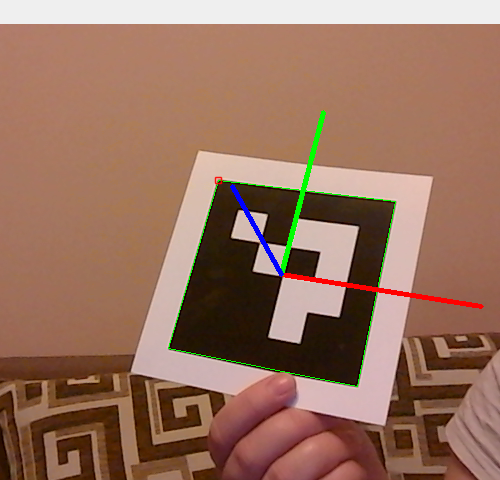
\includegraphics[width=4truecm, height=2.8truecm]{images/felismeres_aruco.png}
	\caption{A demó eredménye}
\end{figure}

\SubSection{A marker felismerésére készített program tesztje:}

A végső programban az ArUco marker felismerés egy olyan függvényként jelenik meg, ami megkap egy képet és ha talál rajta markert, akkor visszaadja a megfelelő vektorokat. (forgás és eltolás)

Ezen programrésznek a tesztelésére készítettem a nyomtatott markeremről pár képet és megnéztem milyen eredményeket ad vissza és felismeri-e a képen szereplő markert.

Azon kijelentés, hogy ha takarásba kerül a marker bármely része, akkor nem lesz továbbá felismerhető teljesen helytálló, hisz legyen bármilyen kicsi az eltakart rész a program nem ismeri fel. 

Az eredmény a vektorokat a fent már említett \texttt{estimatePoseSingleMarkers} adja vissza. 

Az \texttt{rvec} a marker kamerához képest vett elfordulása \texttt{ x, y, z} tengelyeken a \texttt{tvec} pedig a marker eltolása ugyanezekhez. Tehát egy markerhez két vektorhármast kapunk vissza.   

Ezen vektorok fogják a későbbiekben meghatározni a kirajzolandó modellek helyét a térben.

A lentebb szereplő képekhez kapot értékek közül néhány:
\begin{itemize}
\item 1.kép rvec és tvec értékei::
\[[-0.00010618, -0.00181233, 0.04695004]\]
\[[ 1.91320312, -1.6522394,  0.60923043]\]
\item 2.kép rvec és tvec értékei::
\[[-0.00082155,  0.00022395,  0.06280824]\]
\[[ 1.83895896, -1.46640971,  0.69940467]\]
\item 3.kép rvec és tvec értékei:
\[[-0.00619668, 0.00013297,  0.04769506]\]
\[[ 1.87260078 -1.66750728  0.64313328]\]
\item 5.kép rvec és tvec értékei:
\[-0.00501719, -0.01433891,  0.08986719]\]
\[[ 1.25084371,  2.11521712, -1.07834937]\]

\end{itemize}

Látható például, hogy az 5. kép eltolási és forgatási vektorainak értéke nagyobb, mint a 1. vagy 2., hisz ez messzebb van a képen a kamerához képest és jobban el van forgatva, mint a másik kettő.


Természetesen ha nem ismeri fel a amerkert vagy nincs marker a képen 0 add vissza a program.

A képek, ahol felismerte a markert:

\begin{figure}[htp]
    \centering
   	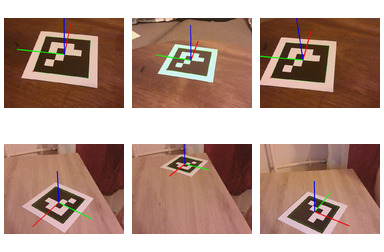
\includegraphics[width=7truecm, height=5truecm]{images/detect.jpg}
	\caption{sikeres detektálás}
\end{figure}

A képek, ahol nem ismerte fel a markert:
\begin{figure}[htp]
    \centering
   	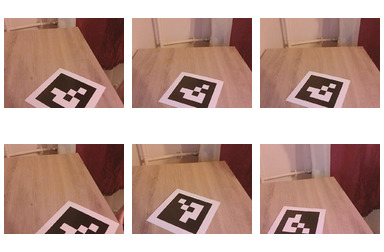
\includegraphics[width=7truecm, height=5truecm]{images/not_detect.jpg}
	\caption{sikertelen detektálás}
\end{figure}
